% Evidence and audit: analyses/024-2026-09-17-h-only-kernel-latency/observations/041-kernel-appendix.md.
% Figure/data: Analysis024/31_kernel_appendix.py; data/kernel-appendix.json.
% Implementation: Run028 candidates/k050, k049, k042, k035; Run035 kernel/.
% Controlled tests: Run037 results/conditional-effects-audit.json; Run039 results/mechanism.json.
\subsection{Kernel development and evaluation}
\label{app:kernel-results}
\label{app:kernel-diagnostics}

\paragraph{Implementation.}
The specialized forward pass preserves each trained model's weights,
thresholds, biases and residual connections. It combines CUDA, CUTLASS and
FlashAttention components to fuse operations and skip matrix instructions
whose activation operands are zero. It introduces no additional pruning.
One kernel computes the two input LayerNorms from their shared input while
retaining separate affine parameters and thresholding. QKV layout conversion,
RoPE and the selected $q,k,v$ gates are fused; $q,k$ gates follow RoPE.
The FFN-down and attention-output projections are evaluated jointly with
their biases and residual addition. The final vocabulary projection remains
dense. Table~\ref{tab:kernel-paths} specifies the sparse execution rules.

\begin{table}[!htb]
\centering\small
\caption{\textbf{Sparse execution rules.} Tile dimensions are tokens by input
features. A matrix multiply--accumulate (MMA) instruction operates on
$16\times8\times16$ elements (output rows, output columns, reduction dimension).
Zero checks and any scalar replacement execute during every forward pass.}
\label{tab:kernel-paths}
\begin{tabularx}{\linewidth}{@{}p{.22\linewidth}XX@{}}
\toprule
Operation & Execution rule & Work avoided \\
\midrule
QKV, FFN-up ($a,m$) & Test each $16\times16$ activation fragment after both
operands have been loaded. & Skip the MMA for an empty fragment; retain operand reads. \\
FFN-down, attention output ($h,z$) & Inspect eight rows; use scalar arithmetic
for rows with at most two nonzeros when numerical guards pass. Process the
remaining rows in $8\times16$ tiles padded to 16 rows. & Skip empty tiles
before loading their weights. Scalar rows read only the corresponding weights. \\
Attention ($QK,PV$) & After loading the operands, use a warp-wide check to
test whether either complete MMA fragment is zero. & Skip that MMA; retain
input loading, masking, softmax and output processing. \\
\bottomrule
\end{tabularx}
\end{table}

The scalar path requires finite weights and biases, with nonzero magnitudes
between $2^{-50}$ and $2^{50}$; selected activations obey the same magnitude
bounds. Other rows use the matrix path. The two sizes retain these rules,
with projection dimensions adapted from $(d,d_f)=(128,512)$ to $(512,2048)$.
The 14M attention kernel uses $64\times256$ query/key tiles and two key/value
partitions; 70M uses $128\times128$ tiles without partitioning to match its
native attention reduction order. This change was needed for numerical
agreement, rather than selected by a 70M performance search.

\paragraph{Scope and numerical checks.}
Tests use one RTX\,5090, BF16 inference, batch size one, 2,048-token causal
sequences, and all 50,304 output logits, with PyTorch 2.11.0, Transformers
5.12.1 and CUDA 12.8. The implementation assumes fixed weights, shapes and
non-overlapping use of its buffers. It is not evaluated for training, cached
decoding, concurrent serving, arbitrary masks or thresholds outside the tested
grid. Each final checkpoint must pass in three fresh processes on all 338
validation sequences. Relative to the unmodified eager implementation, outputs
must be finite, every logit must satisfy
$|y-\hat y|\leq0.25+0.02|\hat y|$, the relative $\ell_2$ error of each sequence's
logits must not exceed $0.02$, and the absolute mean validation-loss difference
must not exceed $0.001$. These are numerical tolerances, not bitwise equivalence.

\paragraph{Timing and reference.}
Native PyTorch/SDPA and specialized inference use CUDA graphs with identical
inputs. Latency is the geometric mean of host timings over 64 fixed validation
sequences, seven randomized paired passes and three fresh processes.
Compilation, static weight layout preparation, graph capture and equal input
staging are excluded. Embeddings, all blocks, final normalization, vocabulary
logits and input-dependent preprocessing are included. Post-hoc masks also
remain inside timing; no activations are cached. Measurements use separate
GPU sessions, so common normalization does not remove session effects.

For comparisons across recipes, Figure~\ref{fig:kernel-diagnostics} uses
\emph{one native base-model latency per size}:
$t_{\mathrm{native},T_0/P_0}/t_{\mathrm{specialized},r}$ for recipe $r$.
The native references are 0.65544\,ms at 14M and 1.66388\,ms at 70M.
This differs from Figure~\ref{fig:base-model-speedup}, which uses the
specialized base-model latencies, 0.65157 and 3.31325\,ms.
The best trained-recipe gains are therefore $1.427\times$ and $1.028\times$
over the native base, versus $1.418\times$ and $2.047\times$ over the
specialized base. The latter 70M ratio reflects a slow dense path in the
ported implementation and does not establish a twofold gain over native inference.

\paragraph{What MMA bypass measures.}
Bypass is the number of omitted MMA instructions divided by issued plus
omitted instructions, pooling integer counts across layers and validation
sequences. Projection totals pool the four projection operations; attention
totals pool $QK$ and $PV$. We keep the two groups separate because equal
instruction counts need not imply equal costs. At $h,z$, bypass includes
replacement by scalar arithmetic and counts padded rows; it is not a fraction
of all arithmetic eliminated. Attention counts include causal padding:
even the base model bypasses $10.42\%$ of $PV$ instructions at 14M and
$5.15\%$ at 70M. In contrast, $\Smodel$ excludes masked pairs and includes
the dense vocabulary projection in its denominator.

The figure's projection scalar sparsity pools zero-activation products over
all projection products in the actual BF16 operands. Both this measure and
bypass cover all 338 validation sequences; timing uses the 64-sequence subset.
Thus these diagnostics complement, rather than redefine, the canonical
model-wide sparsity used in the quality figures.

\begin{figure}[!htb]
\centering
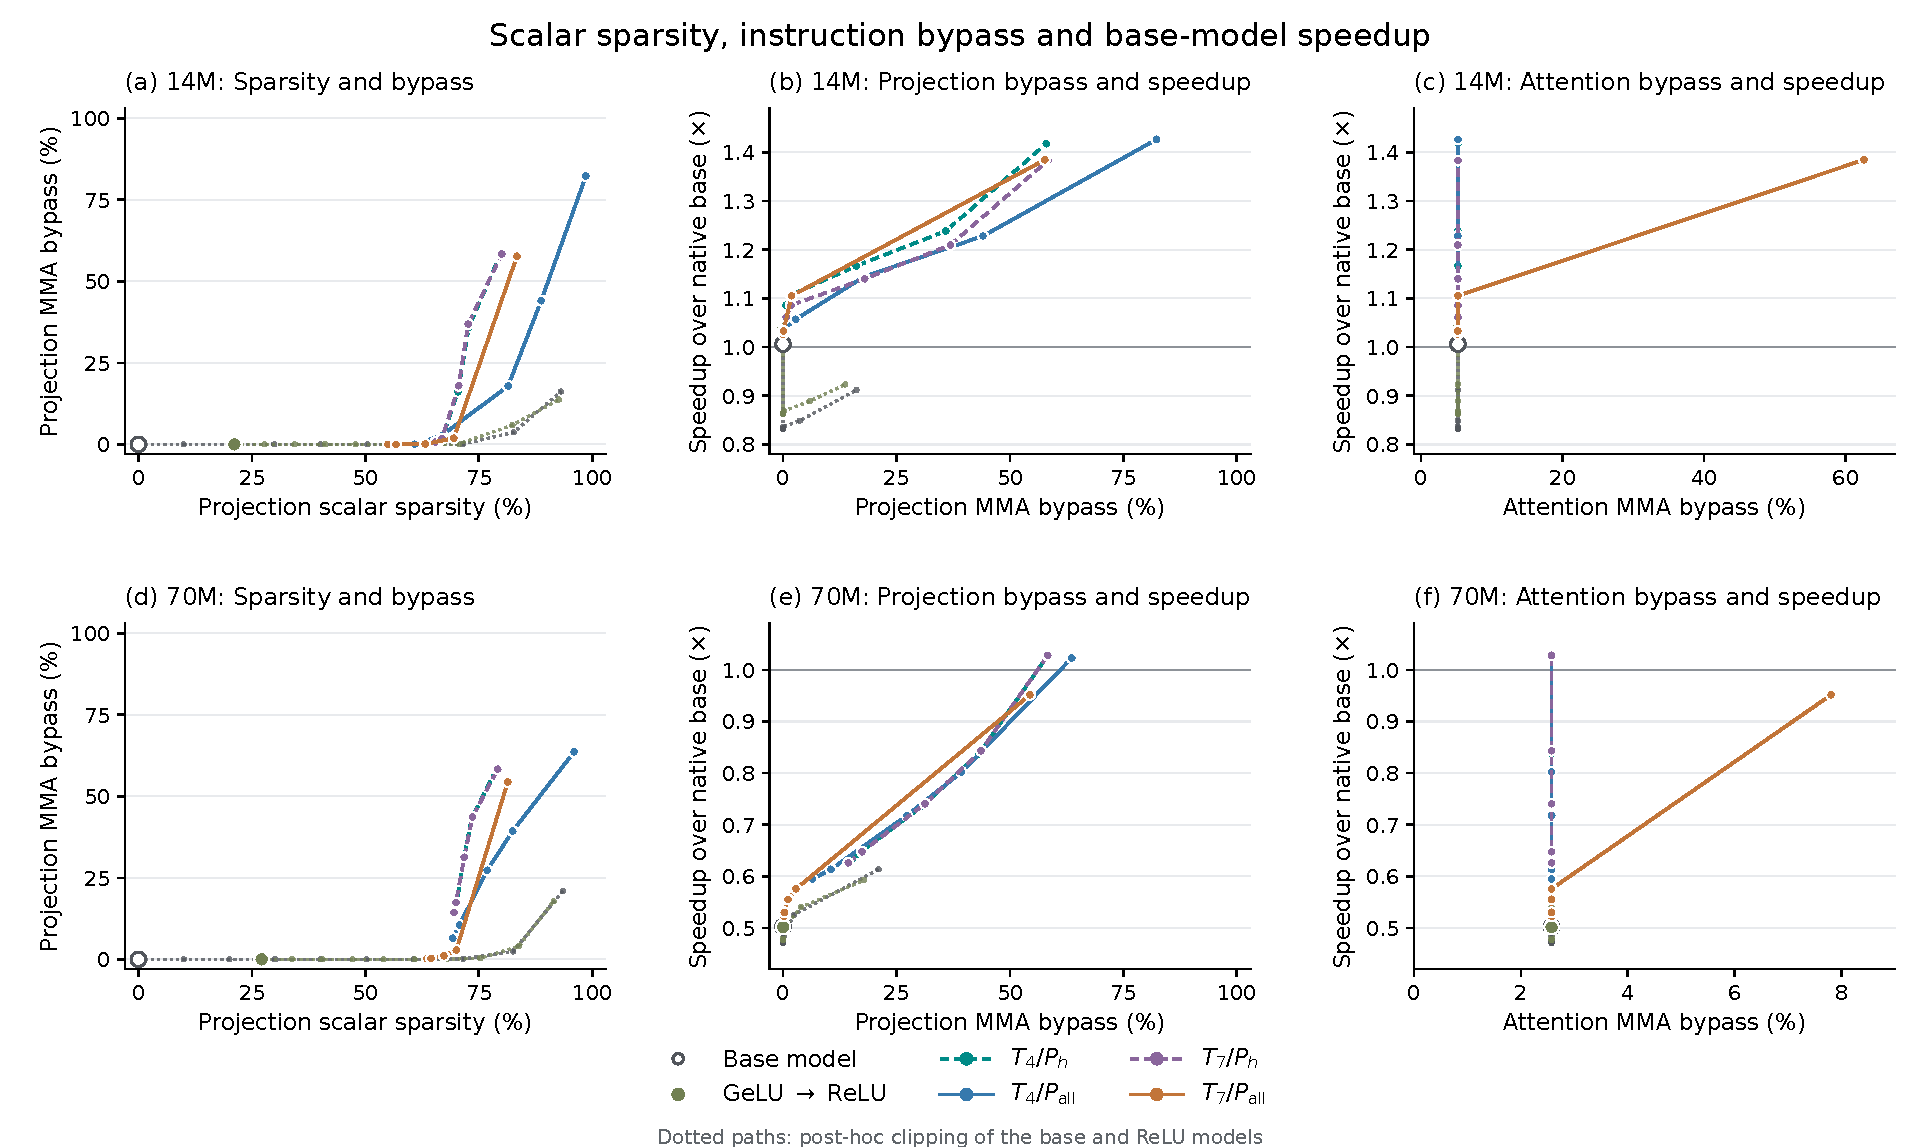
\includegraphics[width=\linewidth]{figures/20-kernel-structure-native-base-speedup.pdf}
\caption{\textbf{Scalar sparsity, instruction bypass and speedup over a fixed
native base model.} Rows show 14M and 70M, each with 22 trained settings and
20 post-hoc control settings. Left: projection scalar sparsity versus projection
MMA bypass. Middle/right: projection/attention bypass versus full-model speedup.
Every speedup within a row uses the same native $T_0/P_0$ reference; the
horizontal line is $1\times$. The Base model marker uses specialized inference,
so it need not lie on that line. Lines connect measured thresholds, not fitted
trends; dotted paths are post-hoc clipping. Counts are pooled, include the
instruction-padding and scalar-substitution conventions above, and do not
measure saved memory traffic.}
\label{fig:kernel-diagnostics}
\end{figure}

\paragraph{Interpretation and controlled tests.}
Projection bypass tracks speedup in both sizes, but high scalar sparsity alone
need not produce empty instruction tiles. Post-hoc controls show this gap and
incur separate masking costs. Attention bypass is nearly constant across the
trained grid except for $T_7/P_{\mathrm{all}}$ at $\kappa=0.5$; this single
exception cannot establish a general attention-speedup relation. At 70M it
has more attention bypass but less native-base speedup than $T_7/P_h$
($0.952\times$ versus $1.028\times$). Bypass therefore describes exploitable
structure without explaining all latency differences.

Table~\ref{tab:kernel-mechanisms} provides the direct 14M test: disable one
skipping path while keeping weights, gates and fusion fixed. Its min--max
spans cover all pairs of three independent off/on process means; effects are
conditional and non-additive. These tests do not separately time memory reads,
zero checks or softmax. No corresponding operation-level ablation was run at
70M, so its scatter is descriptive evidence, not causal attribution.

\paragraph{Alternatives tested.}
Porting the $h,z$ strategy to $a,m$ was correct but slower in the tested 14M
case (Section~\ref{sec:kernel-autoresearch}). The padded fallback issued
$1.90\times$ and $2.00\times$ as many matrix instructions, respectively.
Attention shortcuts using cumulative value sums for zero queries, disjoint
query/key supports, or cheaper conditional execution either failed numerical
checks or did not establish a reliable gain. Disabling attention skipping
improved all 35 historical 14M comparisons. The retained implementation is
therefore not latency-optimal; it preserves one common execution policy across
recipes. Earlier detection that avoids attention operand reads, fused post-hoc
masking and sparsification of softmax probabilities remain untested here.
